\documentclass[a4paper,10pt]{article}

% Paquetes requeridos
\usepackage[utf8]{inputenc}
\usepackage[T1]{fontenc}
\usepackage[spanish]{babel}
\usepackage{csquotes}
\usepackage{amsmath, amssymb, amsfonts}
\usepackage{graphicx}
\usepackage[style=apa, backend=biber, natbib=true, language=spanish, url=true]{biblatex}
\usepackage{tocloft} % Para personalizar el índice
\usepackage[left=3.5cm,right=2.5cm,top=3.5cm,bottom=3.8cm]{geometry}
\usepackage{setspace} % Espaciado
\usepackage{titlesec} % Para personalizar los títulos
\usepackage{fancyhdr} % Para personalizar encabezados y pies de página
\usepackage{newtxtext}
\usepackage{ragged2e}
\usepackage{caption}
\usepackage{parskip} % para que no indente los párrafos
\usepackage{footnote}

\makesavenoteenv{figure}
% Configuración para las etiquetas de figura
\captionsetup[figure]{labelformat=empty} % Esto elimina el número de figura y el separador

\pagestyle{fancy}
\fancyhf{} % Limpia encabezados y pies de página
\renewcommand{\headrulewidth}{0pt} % Elimina la línea del encabezado
% Configuración para las etiquetas de figura
\captionsetup[figure]{labelformat=empty} % Esto elimina el número de figura y el separador

\addbibresource{referencias.bib}
\DeclareLanguageMapping{spanish}{spanish-apa}
% Configuraciones
\setlength{\parskip}{6pt} % Espacio entre párrafos
\setstretch{1.15} % Espacio entre líneas

\renewcommand{\cftsecleader}{\cftdotfill{\cftdotsep}} % Para puntos en el índice

% Estilos para títulos y subtítulos
\titleformat{\section}
{\normalfont\fontsize{12}{15}\bfseries}{\thesection}{1em}{}
\titleformat{\subsection}
{\normalfont\fontsize{10}{13}\bfseries}{\thesubsection}{1em}{}
\titleformat{\subsubsection}
{\normalfont\fontsize{10.5}{13}\bfseries}{\thesubsubsection}{1em}{}

\usepackage[hypertexnames=false, colorlinks=true, 
linkcolor=blue, 
citecolor=blue, 
urlcolor=blue, 
linkbordercolor={1 1 0}, 
citebordercolor={1 1 0}, 
urlbordercolor={1 1 0}, 
filecolor=blue, 
pdfborderstyle={/S/U/W 1}]{hyperref}

% Inicio del documento
\begin{document}
	% Carátula
	\centering
	{\fontsize{14}{17}\bfseries Criptografía ligera: conceptos, avances y tendencias en seguridad para IoT y dispositivos con recursos limitados\par}
	{\small Borgo, Martín Alejandro; Molina, Leandro Rodrigo; Reniero, Oscar Isaías\par}
	{\normalsize Universidad Nacional de Entre Ríos\par}
	{\normalsize Facultad de Ciencias de la Administración\par}
	{\normalsize Licenciatura en Sistemas\par}
	{\small \href{mailto:martinborgo8@gmail.com}{martinborgo8@gmail.com}, \href{mailto:LeandroRodrigoMolina@gmail.com}{LeandroRodrigoMolina@gmail.com}, \href{mailto:isa.reniero001@hotmail.com}{isa.reniero001@hotmail.com}\par}	
	% Resumen y palabras clave
	{\begin{quote} \small \justify \textbf{Abstract.} La criptografía ligera, es una rama de la criptografía que se enfoca en desarrollar algoritmos eficientes y de bajo consumo para su implementación en sistemas con recursos limitados, como sistemas embebidos, dispositivos IoT y microcontroladores. La ausencia de medidas de seguridad adecuadas en tales sistemas genera preocupaciones, especialmente cuando se trata de gestionar información sensible. En este contexto, la criptografía ligera ofrece soluciones que permiten proteger eficazmente los datos y las comunicaciones, sin sacrificar la eficiencia de los recursos. En este artículo se recopilan los distintos conceptos, avances y tendencias que se fueron dando a lo largo de los años en este campo de la criptografía.\end{quote} \par}
	{\begin{quote} \small \justify  \textbf{Keywords:} Criptografía ligera, Internet de las Cosas, Seguridad, Algoritmos Livianos. \end{quote} \par}
	
	\justifying
	\section{Introducción}
	\label{seccion1}
	La criptografía ligera es uno de los temas de la actualidad que se encuentra en auge, es usada en dispositivos donde su poder de cómputo es reducido, a este tipo de dispositivos se les conoce como IoT (Internet de las Cosas), aunque en sus inicios recibía el nombre de red de sensores. Muchos de estos dispositivos utilizan microcontroladores de muy bajo consumo que solo pueden permitirse una pequeña parte de su cómputo a la seguridad\footnote{Es importante tener en cuenta que, aunque la criptografía ligera es útil para dispositivos con recursos limitados, los avances en la tecnología a menudo influyen en lo que se considera 'ligero'. Ya que lo que se considera ligero en un momento dado podría no serlo en un futuro, a medida que la capacidad de los dispositivos mejore.}. Por lo que, los algoritmos de criptografía avanzada no puedan ser usados debido a su alta latencia y consumo de energía. La criptografía ligera nos brinda una gran variedad de algoritmos ‘livianos’ que han sido diseñados para garantizar confidencialidad, autenticidad e integridad de los datos en los dispositivos IoT. Si bien estos algoritmos han sido desarrollados en distintos ámbitos, en sus inicios eran empleados principalmente en el área industrial, un ejemplo común de este uso es el de las redes de sensores, cuyo objetivo es conectar grandes cantidades de sensores muy simples a un centro principal. Estos sensores funcionan con baterías y/o generando su propia energía utilizando, por ejemplo, paneles solares. Los algoritmos criptográficos se emplean normalmente en los canales de comunicación entre los sensores y su centro para proporcionar seguridad, autenticidad e integridad de los mensajes. Sin embargo, debido a la muy baja energía disponible y porque la seguridad es un gasto adicional a la funcionalidad real del dispositivo, los algoritmos criptográficos deben ser lo más ‘pequeños’ posible \parencite[1]{biryukov2017state}. Con el transcurso del tiempo, la aplicación de estos algoritmos se expandió a diversas áreas, como el sector médico y el de los dispositivos electrónicos, tales como televisores y lavadoras, entre muchos otros \parencite{thakor2020lightweight}.
	
	Debido a la gran relevancia que estaban adquiriendo este tipo de algoritmos de encriptación, en 2011 se estandarizan gran parte de estos a través de la creación de la ISO/IEC 18033, que en sus diferentes incisos quedan descritos y especificados cada uno de los métodos de encriptación que estaban siendo utilizados a nivel industrial, académico y gubernamental hasta día de hoy. Sin embargo, el paso más grande se dio en 2012 con la salida de la ISO/IEC 29192-1:2012 donde se introduce por primera vez el término criptografía ligera, brindando definiciones y estableciendo una serie de requerimientos de seguridad, implementación y clasificación. De la mano de la estandarización vienen un conjunto de ventajas, de las cuales \textcite{eterovic15stream} mencionan las siguientes:
	\begin{enumerate}
		\item La libre disponibilidad del algoritmo para su uso, lo que permite que los algoritmos estén disponibles de manera libre para ser utilizados por diversas entidades, facilitando su acceso y aplicación en diferentes sectores.
		\item Contar con una descripción detallada de las funciones que lo conforman, como así también del diseño en general. Esto asegura que las entidades que implementen estos algoritmos tengan acceso a información completa y precisa sobre cómo utilizarlos y aplicarlos de manera efectiva.
		\item La posibilidad de realizar una verificación del funcionamiento y conformidad por parte de un equipo independiente de expertos, permite asegurar que los algoritmos sean robustos y cumplan con las expectativas y normativas establecidas.
		\item La existencia de vectores de prueba\footnote{Los vectores de pruebas son un conjunto de datos de entrada predefinidos y conocidos, utilizados para probar y verificar el correcto funcionamiento de un algoritmo.} garantiza que los algoritmos puedan ser corroborados y validados en cuanto a su buen funcionamiento, proporcionando una capa adicional de confianza y seguridad en su implementación.
	\end{enumerate}
	
	En consecuencia, en los últimos años se ha experimentado un significativo progreso no sólo en la identificación de vulnerabilidades sino también en la corrección de éstas y en la invención de nuevos métodos de encriptación, un caso de esto es el trabajo realizado por \textcite{gunathilake2019next}, el cual menciona los usos actuales de estos algoritmos, además de nombrar cuáles son los mejores a utilizar en las redes 5G. \textcite{eterovic2019criptografia}, por otro lado, realiza una recopilación de algoritmos ligeros utilizados actualmente en el sector comercial, describiendo sus principales características y los ataques a los que fue sometido cada uno de estos, y finaliza su artículo dando una serie de pautas a tener en cuenta al momento del diseño de estos algoritmos.
	
	Este artículo se enfocará en llevar a cabo un análisis preliminar sobre esta subárea de la criptografía, abordando conceptos, progresos y tendencias actuales en el desarrollo de este tipo de algoritmos. En la sección \ref{seccion2}, se realizará una exploración del campo de la criptografía ligera, explicando las diversas clasificaciones y consideraciones propias de diseño, además de nombrar las tendencias que están siendo adoptadas en la construcción de este tipo de algoritmos. En la sección \ref{seccion3}, se abordarán los resultados obtenidos de la revisión bibliográfica. Por último, en la sección \ref{seccion4}, se presentarán las conclusiones obtenidas y las líneas de investigación propuestas.
	
	\section{Clasificación y consideraciones en el diseño}
	\label{seccion2}
	Esta sección exhibe los métodos principales de cifrado de datos, abarcando tanto los cifrados simétricos como asimétricos. Luego, se exploran los tipos de implementación de estos algoritmos: software y hardware. Finalizando, se analizan los aspectos que los diseñadores deben tener en cuenta al llevar a cabo estas implementaciones.
	
	\textcite{wehbe2022criptografia} realiza una clasificación de los distintos algoritmos de encriptación, dividiéndolos en 4 grandes grupos:
	\begin{enumerate}
		\item \textbf{Stream ciphers: }Es un cifrado simétrico que opera con una transformación que varía con el tiempo en dígitos individuales de texto plano. Una secuencia de texto plano se cifra usando una secuencia pseudoaleatoria, generada a partir de una clave secreta y un parámetro público. Cada dígito cifrado se obtiene combinando el dígito correspondiente de texto plano con esta secuencia.
		\item \textbf{Block ciphers:} Es un cifrado simétrico que, para una clave específica $k$, define un algoritmo de cifrado que convierte un bloque de texto plano de $n$ bits en un bloque de texto cifrado de $n$ bits, y un algoritmo de descifrado correspondiente.
		\item \textbf{Funciones de hashing: }Toman cadenas de entrada de longitud arbitraria y las convierten en cadenas de salida de longitud fija y corta, que es única para cada entrada.
		\item \textbf{Algoritmos de criptografía asimétrica:} Utiliza claves diferentes para cifrar y descifrar. Una clave puede ser pública, mientras que su contraparte debe mantenerse en secreto. Incluye algoritmos como RSA (Rivest, Shamir y Adleman) el cual se basa en la dificultad de factorizar grandes números enteros, o las curvas elípticas que permite utilizar claves más cortas y realizar cálculos menos intensivos, siendo óptima para entornos con recursos limitados.
	\end{enumerate}
	
	En la actualidad se proponen muchos algoritmos criptográficos donde sus diseños varían, y cuya única similitud es la baja potencia requerida para su ejecución. La implementación o diseño de estos algoritmos están divididos en dos: hardware y software. Independientemente de la forma de implementación, al momento de su diseño se debe hacer hincapié en aspectos como: el consumo de memoria, el tamaño de la implementación (código o circuito requerido) y la velocidad del algoritmo. La única diferencia entre ambas implementaciones son los parámetros utilizados para indicar su eficiencia. A continuación, se mencionan los aspectos principales en los que se deben enfocar cada uno de los diseñadores e implementadores de acuerdo con el tipo de implementación particular por la que se haya decantado.
	
	Si se desea realizar una implementación por hardware, para que este sea eficiente se deben tener en consideración los siguientes puntos:
	\begin{itemize}
		\item Se debe minimizar el consumo de memoria, RAM o el área de puerta (Gate Area)\footnote{Hace referencia al espacio que un circuito ocupa en un chip, medido por el número de funciones lógicas básicas (AND, OR, XOR, etc) o ‘puertas’ que utiliza. Menos puertas generalmente implican menores tamaño y consumo de energía.}, del dispositivo.
		\item La implementación debe ser optimizada, es decir, el diseño debe ser lo más compacto posible para ocupar menos espacio en el chip.
		\item Se debe considerar el acceso a la memoria no volátil y cómo se accede a las claves almacenadas en ella.
		\item Las operaciones como las permutaciones de bits, que son baratas en hardware, son las más preferidas.
		\item La estructura de la clave no debe requerir un estado de clave que se actualice en cada ronda, ya que esto sería costoso en términos de área de puerta.
	\end{itemize}
	Si la implementación que se desea realizar es por software, para que este sea eficiente se deberá considerar los siguientes puntos:
	\begin{itemize}
		\item Se debe minimizar el consumo de memoria (RAM) utilizada.
		\item Las operaciones como las rotaciones de palabras, que son eficientes en software, son preferidas.
		\item Se debe considerar la forma en que se accede a las claves y cómo se almacenan en la memoria.
		\item Las operaciones que son inherentemente costosas en software, como el manejo de bits a nivel individual, deben evitarse o minimizarse.
		\item Las estructuras de clave que pueden evaluarse en tiempo de ejecución, en lugar de recalculadas y almacenadas, son preferibles para mantener la eficiencia.
	\end{itemize}
	Para realizar un diseño e implementación eficiente se deben tener presentes todos los puntos antes mencionados, e independientemente del tipo de implementación por la que se haya optado, un algoritmo debe, idealmente, obtener un equilibrio entre seguridad, rendimiento y costo.
	\subsection{Algoritmos criptográficos ligeros: tendencias y desafíos}
	\label{sec.2.1}
	\textcite{biryukov2017state} enumeran algunas de las tendencias que están siendo adoptadas en el diseño de nuevos algoritmos, entre las cuales se encuentran las operaciones no lineales, las operaciones lineales y los esquemas de llaves. El objetivo principal de las distintas técnicas es dotar a los algoritmos de dos propiedades fundamentales: la difusión y la confusión. La difusión se asegura de que cualquier cambio en los datos de entrada se propaguen de manera extensa y compleja al texto cifrado, dificultando la detección de patrones o relaciones entre los datos de entrada y los datos cifrados. Por otro lado, la confusión se encarga de ocultar la relación existente entre la clave utilizada y la salida cifrada, de modo que sea difícil deducir la clave o cualquier información útil sobre ella a partir de la salida cifrada.
	
	Las operaciones no lineales son realmente necesarias en cualquier algoritmo de encriptación, ya que brindan una mayor protección contra ataques de criptoanálisis\footnote{El criptoanálisis se centra en estudiar y analizar los sistemas criptográficos para poder vulnerar su seguridad. Algunas de las técnicas usadas son el reconocimiento de patrones de redundancia de los textos, el averiguar características del algoritmo de cifrado, entre otras.}, ataques de fuerza bruta\footnote{En los ataques de fuerza bruta se trata descubrir la clave utilizada para cifrar la información, probando todas las combinaciones posibles, es un mecanismo útil cuando se sabe que las llaves de cifrado son cortas.} y ataques de canal lateral\footnote{Un ataque de canal lateral se centra en el análisis de la información indirecta que se filtra durante el proceso de cifrado o descifrado, con el objetivo de descubrir información sensible o claves de seguridad. Esta información puede ser la variación en el consumo eléctrico, el tiempo de respuesta del dispositivo, entre otros.}. Dentro de las técnicas nombradas por los autores se encuentran las tablas de consultas (Look-up Table), las cuales se utilizan para realizar operaciones no lineales de manera más eficiente, y gracias a que estas tablas pueden ser implementadas utilizando cajas de sustitución\footnote{Las S-Boxes son funciones booleanas vectoriales no lineales, que toman un número determinado de bits de entrada y los transforman en otro número de bits de salida, que no necesariamente tiene que ser la misma cantidad de bits.} (S-Boxes), permiten que los algoritmos que utilizan esta técnica puedan ser implementados de forma eficiente por hardware y software. Se menciona también a los algoritmos basados en segmentos de bits, que utilizan S-Boxes de manera distinta, permitiéndole realizar operaciones bit a bit, como AND y XOR, en palabras de w bits. Dado que esta tarea requiere un número limitado de operaciones lógicas, los algoritmos que utilizan este método se destacan por su eficiencia en la implementación tanto por software y hardware. Por último, se encuentran los algoritmos basados en ARX (adición, rotación y XOR) que, debido a su simplicidad, eficiencia y a la gran dispersión en los datos que se consigue con ellos, junto con el hecho de que la adición a nivel de software es extremadamente eficiente, hace que los algoritmos basados en ARX se encuentran entre los mejores en cuanto a rendimiento para microcontroladores.
	
	Las operaciones lineales, por otro lado, tienen un rol fundamental, ya que brindan difusión a los algoritmos. Entre las técnicas mencionadas por los autores se encuentran las matrices de dispersión máxima, las cuales proveen una dispersión adecuada de los datos, al mismo tiempo que minimiza el costo computacional, aumentando la protección contra criptoanálisis lineales y diferenciales. La permutación de bits es otro mecanismo que está siendo altamente utilizado en ciertas plataformas, debido a que, en términos generales, su implementación por hardware se puede realizar a bajo costo, con el inconveniente que por el momento son un poco costosas de realizarse a nivel software, es por esta razón que son mayormente empleados por dispositivos RFID y similares. Por último, se hace mención a los algoritmos que se basan en rotación y XOR (RX), estos brindan una difusión apropiada, siendo barato de implementar tanto por software como por hardware, heredando gran parte de las ventajas de los algoritmos basados en ARX, pero a un menor costo.
	
	Los autores finalizan hablando del sistema de claves, y como su elevado consumo en términos de RAM, hace que los diseñadores opten por implementar estos algoritmos utilizando claves de corta extensión, quedando expuestos a ataques de llaves relacionadas\footnote{Los ataques de claves relacionadas son un tipo de ataque criptográfico en el cual se intenta comprometer la seguridad en el cifrado aprovechándose de la relación existente entre las diferentes claves utilizadas en el sistema. Estos ataques se basan en el hecho de que ciertos algoritmos criptográficos pueden exhibir vulnerabilidades cuando se utilizan claves relacionadas de alguna manera específica.} y ataques de fuerza bruta. Si bien en la actualidad existen una serie de algoritmos que son inmunes a este tipo de ataques, esto lo consiguen añadiendo más rondas al momento de encriptar los datos o a través de esquemas de llaves más complejos, en ambos casos, estas alternativas no son muy preferibles a la hora de crear algoritmos. Por esta razón se crean los distintos esquemas de llaves, cuya principal función es diversificar y distribuir la clave principal en subclaves que se utilizan en diferentes rondas o etapas del cifrado para mejorar la seguridad y la resistencia a diversos tipos de ataques. Al momento de la implementación se puede emplear este mecanismo de diversas formas:
	\begin{itemize}
		\item Utilizar una variante más sencilla del esquema de llaves para solventar problemas de seguridad específicos.
		\item Proporcionar una mayor seguridad mediante un esquema de llaves mucho más complejo.
		\item Generar subclaves a partir de una clave maestra, tomando diferentes grupos de bits de la clave.
		\item Utilizar una función de rotación para actualizar el estado de la clave original.
	\end{itemize}
	
	La tabla \ref{algoritmosCriptografiaLigera} presenta algunos de los algoritmos más populares que utilizan las técnicas antes mencionadas. A continuación, se presenta una breve descripción de estas técnicas junto con sus respectivos acrónimos.
	\begin{itemize}
		\item Tabla de consultas (TC): las tablas de consulta (Look-Up Table) son estructuras de datos que almacenan precomputaciones de datos cifrados o hashes junto con sus correspondientes entradas originales.
		\item Segmentos de bits (ASB): los segmentos de bits son porciones de bits perteneciente a una secuencia de datos planos o cifrados, las cuales son utilizadas en operaciones criptográficas para garantizar la confidencialidad y la seguridad de la información, además de permitir realizar operaciones en paralelo al momento del cifrado.
		\item Adición, Rotación y XOR (ARX): utilizan las operaciones de adición, rotación y XOR para mezclar y transformar los datos de entrada en el proceso de cifrado.
		\item Matrices de dispersión máxima (MDS): es una estructura de datos especialmente diseñada para dispersar y mezclar los datos de entrada de manera óptima, son empleadas, sobre todo, en las funciones de mezcla de algunos algoritmos.
		\item Permutación de bits (PB): la permutación de bits es una operación que cambia la posición de los bits dentro de una secuencia de datos, de acuerdo a cierta regla o patrón predefinido al momento del diseño.
		\item Rotación y XOR (RX): Es una versión recortada del ARX, que se utiliza para el mismo propósito, es decir, mezclar y transformar datos de entrada.
		\item Utilizan una variante sencilla del esquema de llaves (AV): son todos aquellos esquemas de llaves que no utilizan estrategias sofisticadas o complejas para el manejo de las claves.
		\item Utilizan esquemas de llaves más elaborados (AEE): son esquemas de llaves mucho más complejos, estos esquemas por lo general utilizan una mayor cantidad de recursos y son empleados por algoritmos criptográficos avanzados.
		\item Generan subclaves a partir de una clave principal (ASP): este tipo de esquemas de llaves permite utilizar una clave principal, a partir de la cual se crean claves secundarias únicas y específicas para diferentes operaciones o rondas.
		\item Cambian el estado de las claves a partir de una función de rotación (AR): en este esquema de llaves se cambia el estado inicial de la clave mediante una función de rotación, esto implica modificar la clave mediante desplazamientos de bits, lo que aumenta la seguridad y la confidencialidad de los algoritmos a un bajo costo.
	\end{itemize}
	\begin{figure}[h]
		\centering
		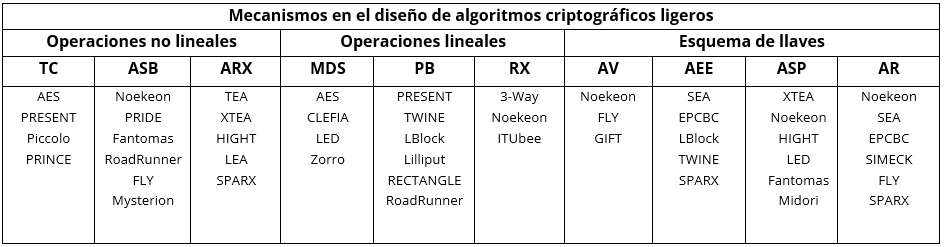
\includegraphics[width=1.0\textwidth]{tablaAlgoritmosCriptografiaLigera.PNG}
		\caption{Tabla 1: Algoritmos populares clasificados según las técnicas que utilizan}
		\label{algoritmosCriptografiaLigera}
	\end{figure}
	
	
	Es importante destacar que algunos de los algoritmos presentes en la tabla pueden pertenecer a más de una categorías debido a múltiples factores, (1) el esquema de llaves es independiente del tipo de técnica utilizada para el cifrado de los datos, (2) ciertos algoritmos hacen uso de diversas técnicas de cifrado al momento de encriptar el texto plano, (3) existen diferentes versiones y/o implementaciones de un mismo algoritmo.
	\section{Resultados obtenidos y esperados}
	\label{seccion3}
	En la sección \ref{seccion2} se clasificó los algoritmos criptográficos en 4 grupos, de acuerdo a la literatura existente. Si bien todos estos esquemas son utilizados para una amplia gama de propósitos, cuando hablamos de algoritmos ligeros, el esquema asimétrico y las funciones hash suelen ser descartadas ya que estos primeros, en términos generales, son muy costosos y las segundas son empleadas para otros tipos de propósitos como la validación de datos o la construcción de primitivos criptográficos. Por esta razón, a la hora de diseñar un algoritmo de estas características se opta por esquemas de encriptación simétrica. En esta sección analizaremos en profundidad los esquemas Block Cipher y Stream Cipher, sus diferencias y aplicaciones.

	 La tabla \ref{Diferencias_Block_Stream_Cipher} detalla las principales diferencias entre ambos modelos de cifrado simétricos. A continuación se describe brevemente qué se aborda en cada una de las columnas.
	\begin{itemize}
		\item Propiedades de los modelos: se abordan las propiedades básicas con las que cuenta cada uno de los modelos, dichas propiedades fueron explicadas en la sección \ref{sec.2.1}.
		\item Uso de la llave: aborda cómo utiliza cada modelo las llaves privadas a la hora de realizar el cifrado del texto plano.
		\item Velocidad: referido al tiempo que le toma a los algoritmos, construidos en cada uno de los modelos, para cifrar el texto plano.
		\item Uso de memoria: referido a la cantidad de memoria utilizada por cada uno de los modelos.
		\item Modo de operación: los modos de operación son las distintas técnicas utilizadas para aplicar los algoritmos de cifrado simétrico a datos de entrada. En este caso, solo se mencionan los más ampliamente utilizados.
		\item Implementación: aborda las dificultades y complejidad a la hora de implementar cada uno de estos modelos.
	\end{itemize}
	\begin{figure}[h]
		\centering
		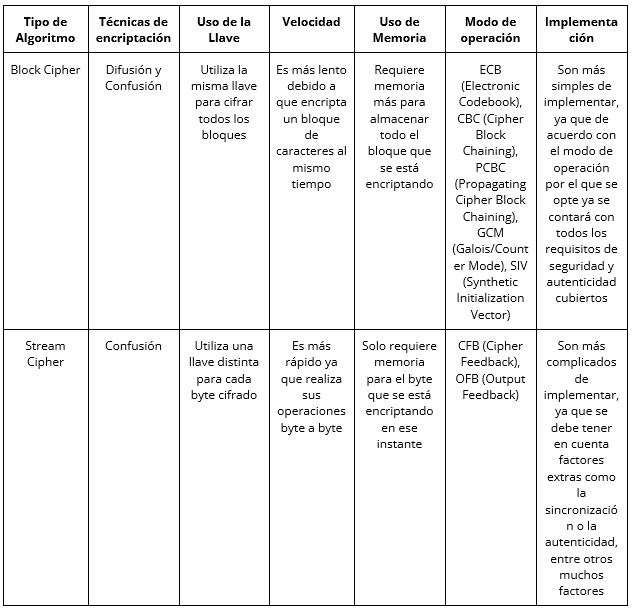
\includegraphics[width=1.0\textwidth]{tablaBlockStreamCipher.PNG}
		\caption{Tabla 2: Diferencias entre modelos de cifrado block cipher y stream cipher.}
		\label{Diferencias_Block_Stream_Cipher}
	\end{figure}
	
	En general se utilizan algoritmos basados en Block Cipher cuando el tamaño de los datos es fijo o es conocido de antemano, se utiliza, por ejemplo, en el protocolo SSL/TLS \parencite{davies2011implementing}. Si bien este protocolo opera de forma híbrida, éste utiliza cifrado de bloque para proteger la comunicación entre el cliente y el servidor. Por otro lado, se utilizan algoritmos basados en Stream Cipher cuando los datos a cifrar poseen un tamaño muy variable e imposible de predecir. Protocolos Wi-Fi como el WEP o WPA e incluso las comunicaciones satelitales utilizan cifrado de flujo.
	
	Estos algoritmos desempeñan un papel importante en diversas áreas, desde la seguridad en comunicaciones hasta aplicaciones en dispositivos inteligentes, logística, agricultura, medicina e industria automotriz. La elección cuidadosa del algoritmo de cifrado es esencial para garantizar la seguridad en una amplia gama de contextos.
	
	\section{Conclusión}
	\label{seccion4}
	En este trabajo, se realizó un breve análisis preliminar del estado actual del conocimiento en el área de la criptografía ligera, abarcando su estandarización mediante las normas ISO/IEC 18033 y 29192, las cuales establecieron una base sólida y uniforme para los diversos algoritmos de encriptación. Además, se ha hecho una clasificación de los distintos grupos de algoritmos, que incluyen Stream/Block Cipher, Hash function y algoritmos asimétricos, destacando sus principales diferencias, usos y en qué situaciones es más conveniente usar cada tipo o familia de algoritmos. Finalizando con los criterios a tener en cuenta al momento de su implementación, ya sea en entornos de software o de hardware. Cabe destacar que el presente trabajo se realizó en el contexto del Proyecto de Investigación propuesto en la asignatura Metodología de la Investigación de 3er año de la carrera de Licenciatura en Sistemas de la Facultad de Ciencias de la Administración.
	
	Como trabajos futuros, se propone el desarrollo y expansión de las siguientes líneas de investigación, logrando profundizar aún más en los temas tratados en este estudio.

	\begin{itemize}
	\item Analizar la eficiencia en cuanto a poder de cómputo y uso de memoria de cada uno de los métodos que pueden ser utilizados para realizar la encriptación, los cuales fueron descritos en la sección \ref{sec.2.1}.
	\item Evaluar las dificultades que se presentan al realizar una implementación por software y por hardware.
	\item Realizar un análisis preliminar de los cifrados híbridos que han ido surgiendo a lo largo del tiempo, explorando su relevancia y ventajas en contextos específicos.
	\end{itemize}
	
	\section{Referencias}
	\nocite{*}
	\printbibliography[heading=none]
\end{document}
